\documentclass[12pt]{article}

\usepackage[letterpaper,margin=1in]{geometry}

\setlength{\parindent}{0pt}

\usepackage{amssymb}
\usepackage{amsmath}

\usepackage{multicol}

\usepackage{tikz}

\newcommand{\headerText}{
  MA 238 | 2019 Spring | Dr. Clontz
}

\usepackage{fancyhdr}
\pagestyle{fancy}
\renewcommand{\headrulewidth}{0pt}% Default \headrulewidth is 0.4pt
\renewcommand{\footrulewidth}{0pt}% Default \footrulewidth is 0pt
\chead{\footnotesize\bf\headerText}
\cfoot{}

\newcommand{\csch}{\operatorname{csch}}
\newcommand{\sech}{\operatorname{sech}}

\newcommand{\issuesMark}{{\fontencoding{U}\fontfamily{futs}\selectfont\char 66\relax}}




\begin{document}


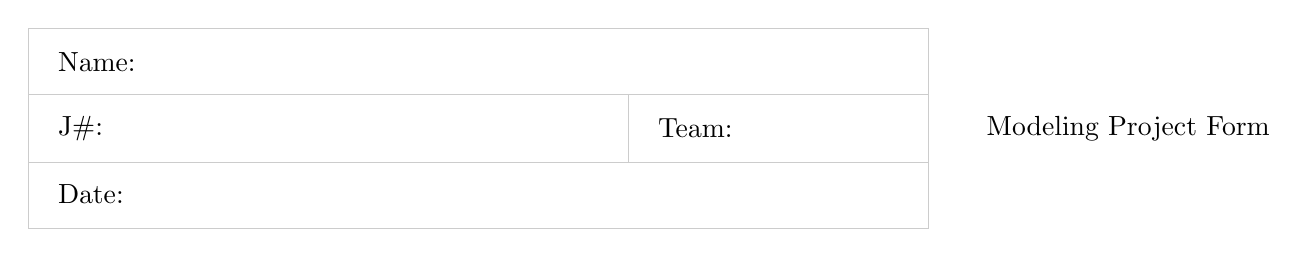
\begin{tikzpicture}[x=1in,y=1in]
  \draw[color=black!20] (0,0) rectangle (4.5,1);
  \draw[color=black!20] (0,0.67) -- (4.5,0.67);
  \draw[color=black!20] (3,0.33) -- (3,0.67);
  \draw[color=black!20] (0,0.33) -- (4.5,0.33);

  \node[anchor=west] at (0.1,0.83) {Name:};
  \node[anchor=west] at (0.1,0.5) {J\#:};
  \node[anchor=west] at (3.1,0.5) {Team:};
  \node[anchor=west] at (0.1,0.17) {Date:};

  \node at (5.5,0.5) {Modeling Project Form};
\end{tikzpicture}

\vspace{1em}

\begin{tikzpicture}[x=1in,y=1in]
  \draw[color=black!50] (0,0) rectangle (6.4,1);
  \draw[color=black!50] (1,0) -- (1,1);
  \draw[color=black!50] (3.2,0) -- (3.2,1);
  \draw[color=black!50] (5.4,0) -- (5.4,1);

  \node[anchor=north west,color=black!70] at (0,0.95) {\footnotesize Standard:};
%  \node[anchor=north west,color=black!70] at (1,0.95) {\footnotesize Mastery Quiz:};
  \node[anchor=north west,color=black!70] at (3.2,0.95) {\footnotesize Exercise Version:};
  \node[anchor=north west,color=black!70] at (5.4,0.95) {\footnotesize Mark:};
\end{tikzpicture}

Write a complete solution (using multiple pages as necessary)
for the exercise version assigned to you from https://mastr.clontz.org .
When complete, scan/upload to the Gradescope app for grading. Revisions are always allowed, so using
a pencil on this form is recommended (or you may use white-out, or choose to reattempt from scratch,
etc.).

\end{document}
